\documentclass{beamer}

\usepackage[utf8]{inputenc}
\usepackage[T1]{fontenc}
\usepackage[ruled,vlined,linesnumbered]{algorithm2e}
\usepackage{tikz}

\usepackage{verbatim}
\usetikzlibrary{arrows,shapes}

\SetAlFnt{\small}
\SetAlCapFnt{\large}
\SetAlCapNameFnt{\large}

%%% algorithm2e environment with "Algoritmi"-caption.
\newenvironment{finalgo}[1][htb]{
  \renewcommand{\algorithmcfname}{Algoritmi}
  \begin{algorithm}[#1]
}{\end{algorithm}}

%%% To be able to not numbering individual lines:
\let\oldnl\nl% Store \nl in \oldnl
\newcommand{\nonl}{\renewcommand{\nl}{\let\nl\oldnl}}

%%% argmin
\DeclareMathOperator*{\argmin}{arg\, min}

\title{{\rmfamily\scshape Lyhimpien polkujen hakualgoritmit ja -järjestelmät}}
\author{$\mathfrak{Rodion \, Efremov}$}
\date{}
\institute{Tietojenkäsittelytieteen laitos, Helsingin yliopisto}

\usetheme{Ilmenau}
\usecolortheme{beaver}
\usefonttheme[onlymath]{serif}

\begin{document}
\maketitle
% Declare layers
\pgfdeclarelayer{background}
\pgfsetlayers{background,main}

%%% BEGIN: Määritelmät
\begin{frame}
  \frametitle{Verkot}
  \begin{itemize}
    \item Suunnattu verkko on $G = (V, A)$, missä $V$ on solmujen joukko ja $A \subset V \times V$ on suunnattujen kaarien joukko.

    \item Suuntaamaton verkko $G = (V, E)$ voidaan aina simuloida suunnatulla verkolla $(V, A)$ laittamalla $A$:han kaaret $(u, v)$ ja $(v, u)$ jokaisella suuntaamattomalla kaarella $\{u, v\} \in E$.

    \item Jatkossa merkitsemme $n = |V|$ ja $m = |E|$.
  \end{itemize}
\end{frame}

\begin{frame}
  \frametitle{Verkot}
  \begin{itemize}
    \item $k$:n kaaren polku on $\gamma = \langle u_0, u_1, \dots, u_k \rangle$, missä kukin solmu esiintyy vain kerran ja jokaisella $i \in \{ 0, 1, \dots, k - 1 \}$ $(u_i, u_{i + 1}) \in A$.

    \item Painotettujen verkkojen kohdalla otaksumme kunkin kaaren $(u, v)$ painon $w(u, v)$ olevan \textbf{ei-negatiivinen}.
    
	\item Polun $\gamma$ paino on $\sum_{i = 0}^{k - 1} w(u_i, u_{i + 1})$.
    
    \item Suuntamattomassa verkossa solmun $u$ ''aste'' on $d(u) = |\{ \{u, v\} \colon \{ u, v \} \in E \}|$. 
    
    \item Suunnatussa verkossa solmun $u$ ''sisäänaste'' (engl. \textit{indegree}) on $\textrm{deg}^-(u) = | \{ (v, u) \colon (v, u) \in A \} |$ ja
      ''ulosaste'' (engl. \textit{outdegree}) on $\textrm{deg}^+(u) = | \{ (u, v) \colon (u, v) \in A \} |$.
  \end{itemize}
\end{frame}
%%% END: Määritelmät

%%% BEGIN: BFS
\begin{frame}
\frametitle{Leveyssuuntainen haku}
\begin{itemize}
\item Löytää lyhimmän polun (yhden monesta mahdollisesta) painottamattomassa verkossa.
\item Toteutus vaatii vain jonon ja hajautustaulun.
\item Toimii ajassa $\mathcal{O}(n + m) \approx \sum_{i = 0}^N d^i$, missä $N$ on lyhimmän polun solmujen määrä ja $d$ keskiarvoinen solmun aste tai solmun ulosaste verkon tyypistä riippuen.
\end{itemize}
\end{frame}
%%% END: BFS

%%% BEGIN: BFS pseudocode
\begin{frame}
\begin{figure}[H]
  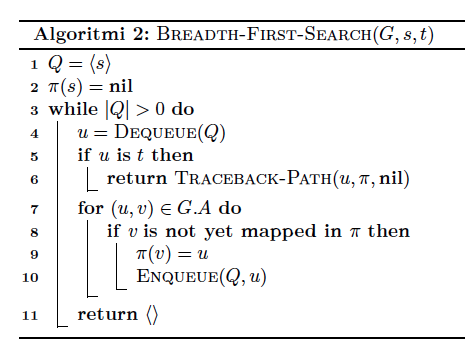
\includegraphics[width=\textwidth,keepaspectratio]{bfs}
\end{figure}
\end{frame}
%%% END: BFS pseudocode

\begin{frame}
Voiko leveyssuuntaisen haun nopeuttaa?
\end{frame}

\begin{frame}
Voi!
\end{frame}

\begin{frame}
\frametitle{Kaksisuuntainen leveyssuuntainen haku}
\begin{itemize}
  \item Aja kaksi hakuavaruutta: yksi normaalin tapaan lähtösolmusta, ja toinen ''takaperin'' maalisolmusta.
  \item Kun kaksi yllä mainittua hakuavaruutta kohtavat jossain ''keskellä'', rakennetaan lyhin polku.
  \item Aikavaativuus on $2\sum_{i = 0}^{\lceil N / 2\rceil} d^i$.
  \item Verkosta riippuen voi olla jopa \textasciitilde 1000 kertaa nopeampi kuin yksisuuntainen BFS.
\end{itemize}
\end{frame}

\begin{frame}
\begin{figure}[H]
  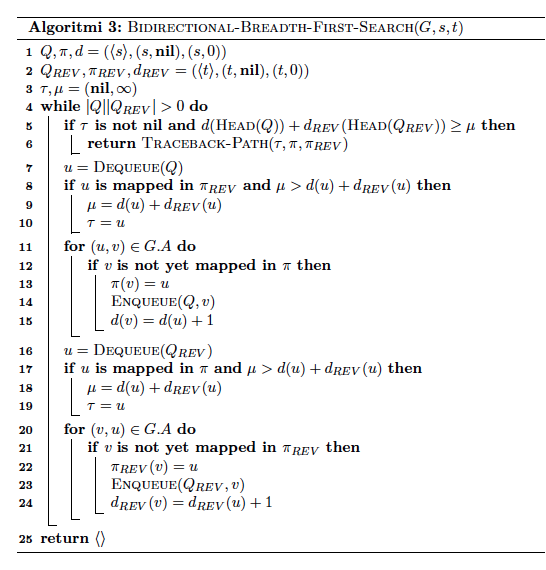
\includegraphics[width=\textwidth,height=\textheight,keepaspectratio]{bibfs}
\end{figure}
\end{frame}

\begin{frame}
Miten rakentaa polut lyhimpien polkujen puusta?
\end{frame}

\begin{frame}
Tarvitaan vain kuvaus $\pi$ (ja myös $\pi_{REV}$ mikäli polku oli haettu kaksisuuntaisella haulla).
\end{frame}

\begin{frame}
  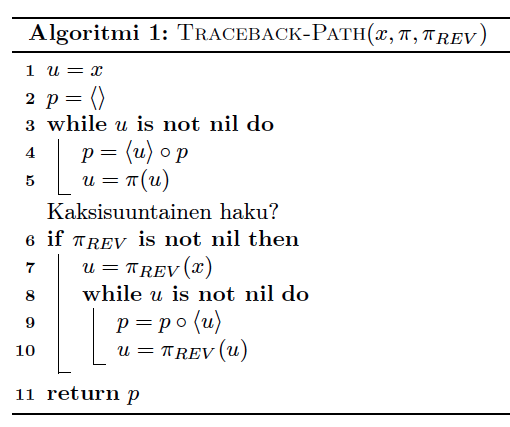
\includegraphics[width=\textwidth,height=\textheight,keepaspectratio]{path}
\end{frame}

\begin{frame}
  \frametitle{Dijkstran algoritmi}
  \begin{itemize}
    \item Vuonna 1959 Edsger W. Dijkstra esitti kuuluisan polunhakualgoritminsa, joka toimii polynomisessa ajassa.
    \item FIFO jonon sijasta prioriteettijono; kutsutaan usein ''avoimeksi'' listaksi (engl. \textit{open set}).
    \item Hajautustauluun perustuva joukkorakenne; kutsutaan usein ''suljetuksi' listaksi (engl. \textit{closed set}).
    \item $g$-kuvaus, joka kuvaa kunkin saavutetun solmun toistaiseksi pienimpään etäisyyteen lähtösolmusta laskettuna.
    \item $\pi$-kuvaus, aivan kuten BFS:ssä (kuvaa solmun edeltäjäänsä lyhimpien polkujen puussa).
    \item Kun solmu poistetaan avoimesta listasta, sen $g$-arvo on optimaali.
  \end{itemize}
\end{frame}

\begin{frame}
  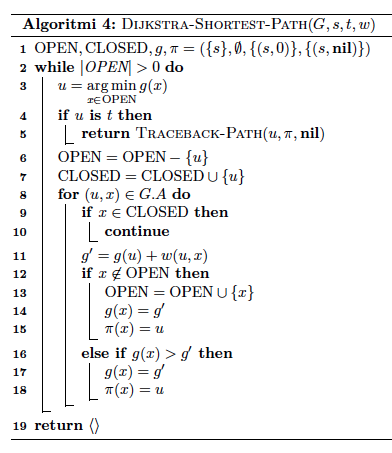
\includegraphics[width=\textwidth,height=\textheight,keepaspectratio]{dijkstra}
\end{frame}

\begin{frame}
  \frametitle{Dijkstran algoritmi}
  \begin{itemize}
    \item Dijkstran algoritmi voidaan mieltää BFS:n yleistykseksi painotetuissa verkoissa: samoin kuten BFS, Dijkstran algoritmi kasvattaa hakuavaruutensa ''kaikkiin suuntiin'' laajenevan pallon tavoin.
  \end{itemize}
\end{frame}

\begin{frame}
  \frametitle{A$\ast$ - haku}
  \begin{itemize}
    \item Pseudokoodi tasan sama kuten Dijkstran algoritmilla, paitsi että rivillä 3 $g(x)$ on korvattava $f(x)$:llä, jolle siis $f(x) = g(x) + h(x)$, missä $h(x)$ on optimistinen (eli aliarvioitu) kustannus solmusta $x$ maalisolmuun.
    
    \item Intuitio järjestelyn takana on se, että A$\ast$ ''tietää'' mihin suuntaan kannattaa lähteä kasvattamaan hakuavaruuden päästääkseen maalisolmuun nopeammin.
    
    \item Määrittämällä $h(u) = 0$ kaikilla $u \in V$, A$\ast$ palautuu Dijkstran algoritmiksi.
  \end{itemize}
\end{frame}

\begin{frame}
  \frametitle{Kaksisuuntainen painotettu haku}
  \begin{itemize}
    \item Myös A$\ast$ ja Dijkstran algoritmit voidaan kaksisuuntaista.
    \item Jos heuristiikkafunktio ei voida määritellä, kaksisuuntainen Dijkstran algoritmi on melkein aina parempit vaihtoehto suhteessa yksisuuntaiseen versioonsa.
    \item Mitä tulee A$\ast$:n kaksisuuntaistamiseen, algoritmi ei nopeudu erityisen paljon, sillä jo ei niin hyvä heuristiikkafunktio karsii hakuavaruuden melko hyvin.
  \end{itemize}
\end{frame}

\begin{frame}
  \frametitle{Kaksisuuntainen Dijkstran algoritmi}
  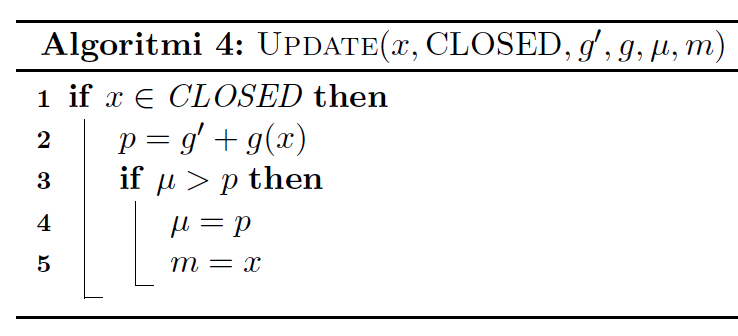
\includegraphics[width=\textwidth,height=\textheight,keepaspectratio]{update}
\end{frame}

\begin{frame}
  \frametitle{Kaksisuuntainen Dijkstran algoritmi}
  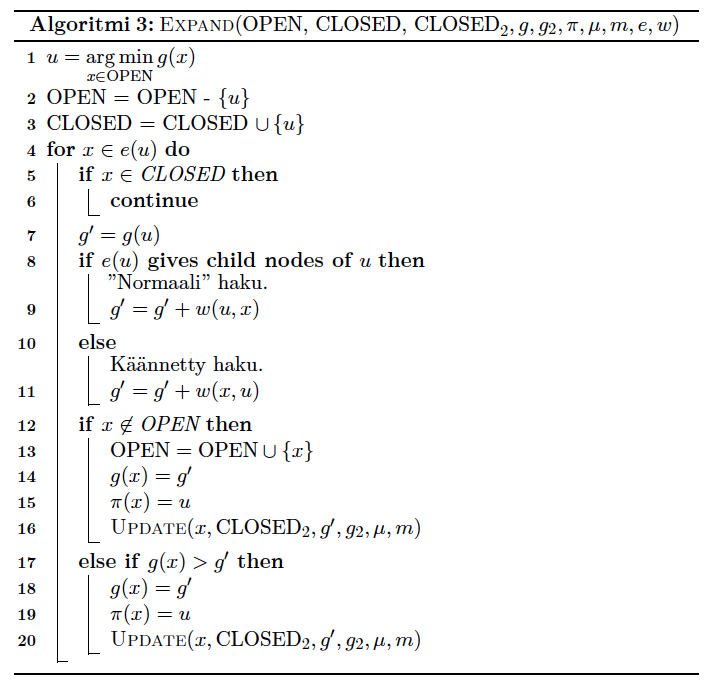
\includegraphics[width=\textwidth,height=0.8\textheight,keepaspectratio]{expand}
\end{frame}

\begin{frame}
  \frametitle{Kaksisuuntainen Dijkstran algoritmi}
  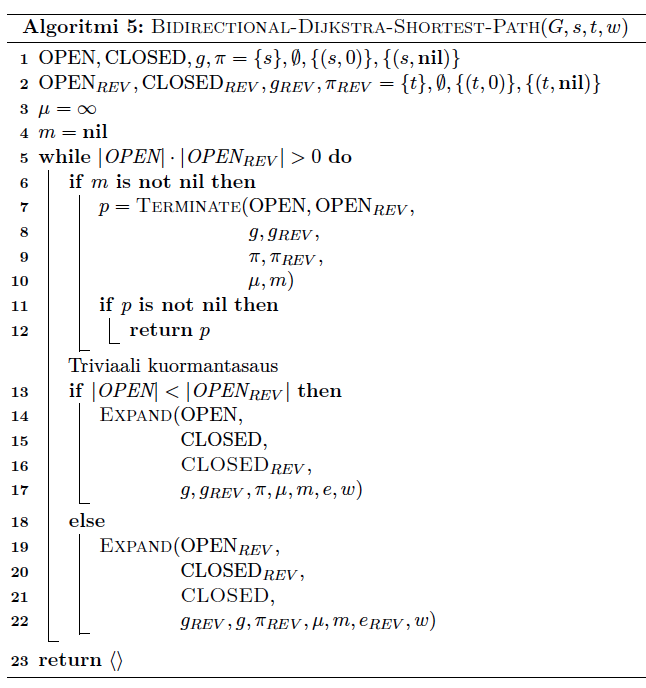
\includegraphics[width=\textwidth,height=0.85\textheight,keepaspectratio]{bidijkstra}
\end{frame}

\begin{frame}
  \frametitle{Kaksisuuntainen Dijkstran algoritmi}
  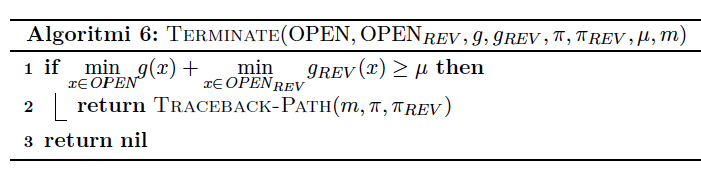
\includegraphics[width=\textwidth,height=0.85\textheight,keepaspectratio]{term}
\end{frame}

\begin{frame}
  \frametitle{Kaksisuuntainen A$\ast$}
  \begin{itemize}
    \item Tasan sama kuin kaksisuuntainen Dijkstra, paitsi että operaation \textsc{Expand} rivillä 1 oleva $g(x)$ korvattava lausekkeella $f(x)$, jolle siis $f(x) = g(x) + h(x)$.
    \item Operaatiossa \textsc{Terminate} testin ehto on
    \[
    \max( \underset{x \in \textsc{OPEN}}{\min} f(x), \underset{x \in \textsc{OPEN}_{REV}}{\min}f_{REV}(x) ) \geq \mu,    
    \]
  \end{itemize}
\end{frame}

\begin{frame}
  Mikä mahtaa olla tehokkain tapaa hakea polut?
\end{frame}

\begin{frame}
  \frametitle{Kaikkien parien lyhimmät polut}
  (1) Aja kaikkien-parit algoritmin, joka palauttaa nk. ''edeltäjämatriisin''.
\end{frame}

\begin{frame}
  \frametitle{Kaikkien parien lyhimmät polut}
  (2) Mikä tahansa $N$:n solmun polku voidaan rakentaa edellä mainitusta matriisista ajassa $\mathcal{O}(N)$!
\end{frame}

\begin{frame}
  \frametitle{Kaikkien parien lyhimmät polut}
  \begin{itemize}
    \item Floyd-Warshall toimii ajassa $\Theta(n^3)$.
    \item Jos $m = o(n^2)$, Johnsonin algoritmi Fibonacci-keolla on asymptoottisesti parempi: $\mathcal{O}(n^2 \log n + nm)$.
    \item Kumpikaan ei siis tarpeeksi tehokas prosessoimaan kokonaisen valtion tieverkkoa, sillä pelkästään solmuja on helposti yli 100000.
  \end{itemize}
\end{frame}

\begin{frame}
  \frametitle{Dijkstran algoritmi kaarivivuilla}
    Jaa kaikki solmut $V$ osituksiin $V_1, \dots, V_k$ siten, että
    \[
      \bigcup_{i = 1}^k V_i = V,
    \]
    ja $V_i \cap V_j = \emptyset$ kaikilla $i \neq j$.
\end{frame}

\begin{frame}
  \frametitle{Dijkstran algoritmi kaarivivuilla}
  $k$ osion ositus voidaan merkitä funktiolla $r \colon V \to \{ 1, 2, \dots, k\}$.
\end{frame}

\begin{frame}
  \frametitle{Dijkstran algoritmi kaarivivuilla}
  Jokaiselle kaarelle asetetaan $k$:n bitin bittivektorin (engl. \textit{arc-flag vector}, kaarivipuvektori); jos $i$des bitti on päällä, kaari on lyhimmällä polulla johonkin osion $V_i$ solmuun.
\end{frame}

\begin{frame}
  \frametitle{Dijkstran algoritmi kaarivivuilla}
  Osion $V_i$ ''rajasolmut'' ovat \[
    B_i = \{ v \in V_i \colon \exists (u, v) \in A \text{ siten että } r(v) \neq r(u) \}.
  \]
\end{frame}

\begin{frame}
  \frametitle{Dijkstran algoritmi kaarivivuilla}
  Jokaisen osion $V_i$ jokaisen rajasolmun $u \in B_i$ lähtien ajetaan ''takaperin'' tavallinen Dijkstra ja tuloksena syntyvässä lyhimpien polkujen puussa $T$ asetetaan jokaisen kaaren $(u, v) \in T$ $i$des vipu päälle.
\end{frame}

\begin{frame}
  \frametitle{Dijkstran algoritmi kaarivivuilla}
  Nyt tuloksena syntyvässä algoritmissa haettaessa polkua solmuun $t \in V$, voidaan karsia kaikki kaaret, joiden $r(t)$:s bitti ei ole päällä.
\end{frame}

\begin{frame}
  \frametitle{Dijkstran algoritmi kaarivivuilla}
  Voidaan myös kaksisuuntaista: jokaisella kaarella kaksi kaarivipuvektoria: yksi normaalia hakusuuntaa varten ja toinen käännettyä hakua varten.
\end{frame}

\begin{frame}
  \frametitle{Dijkstran algoritmi kaarivivuilla}
  Tekniikka voidaan nähdä tasapainoilevan tavallisen Dijkstran algoritmin ($k = 1, V_1 = V$) ja kaikkien parien algoritmin ($k = n$, jokainen solmu on osio) välillä.
\end{frame}

\begin{frame}
  \frametitle{Dijkstran algoritmi kaarivivuilla}
  Tutkijat raportoivat kaksisuuntaisen kaarivipu-Dijkstran olevan keskimäärin yli 500 kertaa nopeampi kuin tavallinen yksisuuntainen Dijkstra.
\end{frame}

\begin{frame}
  \frametitle{Dynaamiset verkot}
  \begin{itemize}
    \item Aiemmin tarkastellut verkot ovat \textbf{staattisia}.
    \item Dynaamisessa verkossa lyhin polku ei riipu vain lähtö- ja maalisolmuista, vaan myös siitä ajasta, jona matka aloitetaan.
    \item Lisäksi, kaarten painot riippuvat siitä, millä ajoneuvoilla ollaan liikkeellä (bussi, raitiovaunu, metro, kävely).
    \item Myös solmuihin liittyy painoja (''Pekka saappui pysäkille, jossa hän odottaa bussin neljä minuuttia.'')
    \item Reittiopas toimii dynaamisilla verkoilla.
  \end{itemize}
\end{frame}

\begin{frame}
  \frametitle{Dynaamiset verkot}
  \begin{itemize}
      \item Jos käyttäjä syöttää lähtöajan, haku on ''normaalia'' lähtösolmusta maalisolmuun.
      \item Jos käyttäjä syöttää saapumisajan, haku on ''käännetty takaperin'' ja etenee ''ajassa taaksepäin'' kunnes kohtaa lähtösolmun.
      \item Kaksisuuntainen haku ei ole dynaamisilla verkoilla mahdollista, sillä se vaatii maalisolmun saapumisajankohdan, jonka voi laskea vain ajamalla yksisuuntaisen haun lähtösolmusta.
  \end{itemize}
\end{frame}

\begin{frame}
  Kiitos!
\end{frame}

\begin{frame}
  Kysymyksiä?
\end{frame}

\end{document}